%
% CHAPTER Versuch 2
%
\chapter{Frequenzgang von Lautsprechern}
Es gilt für zwei Lautsprecher die Amplitude und Phasenverschiebung eines akustischen Signales festzustellen.

\label{chap:FrequenzgangVonLautsprechern}

\section{Fragestellung, Messprinzip, Aufbau, Messmittel}
Um den Frequenzgang eines Lautsprechers zu ermitteln werden Sinussignale mit verschiedenen Frequenzen an diesen angelegt. Die Amplitude eines Signals sollte stets dieselbe sein. Das Signal wird mit einem Sinusgenerator erzeugt und an den Lautsprecher angelegt. Dieses Signal wird an einem Kanal im Oszilloskop gemessen. Der Ton der dabei entsteht wird mit einem Mikrofon aufgenommen und ebenfalls an einem Kanal des Oszilloskops gemessen. Das Mikrofon sollte möglichst stets den gleichen Abstand zum Lautsprecher haben.
Für diesen Versuch werden 17 Messungen, mit unterschiedlichen Frequenzen pro Lautsprecher, gemacht.
Das erzeugte Sinussignal gilt als Referenzwert welches bei jeder Messung eine Amplitude von 1,5V besitzt.
Beim Vergleichen beider Werte sollte sowohl eine Phasenverschiebung als auch ein Amplitudenunterschied festgestellt werden. Dazu später mehr.
Die einzelnen Messungen werden mit folgenden Frequenzen durchgeführt: 
\begin{table}
\begin{tabular}{|c|c|c|}
100 & 850  & 3000 \\
200 & 1000 & 4000 \\
300 & 1200 & 5000 \\
400 & 1500 & 6000 \\
500 & 1700 & 10000 \\
700 & 2000 & \\
\end{tabular}
\centering
\label{tab:Frequences}
\caption{Frequenzen zur Frequenzgangmessung}
\end{table}
Die Messungen werden im "Single Sequence Mode" durchgeführt, um einen Signalausschnitt zu erlangen.
Bei jeder Messung wird sowohl die Amplitude des Ausgangssignals, als auch die Phasenverschiebung gemessen und protokolliert. \ref{} TODO
\label{chap:VERSUCH_2_FRAGESTELLUNG}

\section{Messwerte}
\label{chap:VERSUCH_2_MESSWERTE}
\begin{table}[H]
\centering
\begin{tabular}{ccc}
  Frequenz in $Hz$ & Amplitude in $mV$ &  Phasenverschiebung in $°$ \\
  100 & 50.2 & $-3.60$ \\
  200 & 134.0 & $-578.88$ \\
  300 & 95.2 & $-547,20$ \\
  400 & 60.4 & $-504$ \\
  500 & 49.2 & $-493.2$ \\
  700 & 39.6 & $-490.03$ \\
  850 & 43.2 & $-482.40$ \\
  1000 & 42.0 & $-469.44$ \\
  1200 & 35.2 & $-460.22$ \\
  1500 & 33.6 & $-444.24$ \\
  1700 & 30.8 & $-437.11$ \\
  2000 & 32.0 & $-421.92$ \\
  3000 & 37.6 & $-414.00$ \\
  4000 & 46.0 & $-1054.008$ \\
  5000 & 26.8 & $-982.80$ \\
  6000 & 19.4 & $-974.88$ \\
  10000 & 15.4 & $-752.40$ \\
 \end{tabular}
\label{tab:MLg}
\caption{Messwerte Lautsprecher groß}
\end{table}

\begin{table}[H]
\centering
\begin{tabular}{ccc}
  Frequenz in $Hz$ & Amplitude in $mV$ &  Phasenverschiebung in $°$ \\
  100 &  6.6& $-50.40$ \\
  200 & 10.4 & $-380.16$ \\
  300 & 15.0 & $-409.68$ \\
  400 & 23.8 & $-436.32$ \\
  500 & 34.6 & $-442.80$ \\
  700 & 70.0 & $-501.12$ \\
  850 & 68.0 & $-574.20$ \\
  1000 & 50.0 & $-471.60$ \\
  1200 & 40.0 & $-463.68$ \\
  1500 & 52.8 & $-509.04$ \\
  1700 & 53.6 & $-445.68$ \\
  2000 & 51.2 & $-432.00$ \\
  3000 & 50.4 & $-394.56$ \\
  4000 & 52.0 & $-1028.16$ \\
  5000 & 12.8 & $-1022.4$ \\
  6000 & 8.2 & $-914.40$ \\
  10000 & 19.4 & $-727.20$ \\
 \end{tabular}
\label{tab:MLk}
\caption{Messwerte Lautsprecher klein}
\end{table}

\begin{figure}[H]
\centering
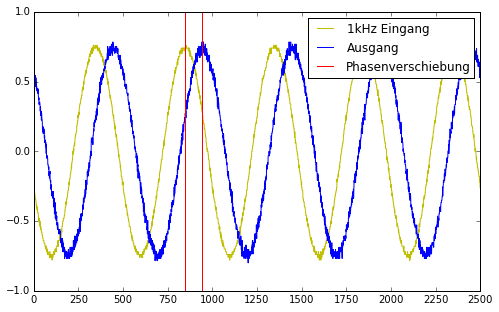
\includegraphics[width=165mm]{ein-ausgang.png}
\caption{Eingangsignal Lautsprecher und Ausgangssignal Mikrofon}
\label{img:EingangAusgang}
\end{figure}

\begin{figure}[H]
\centering
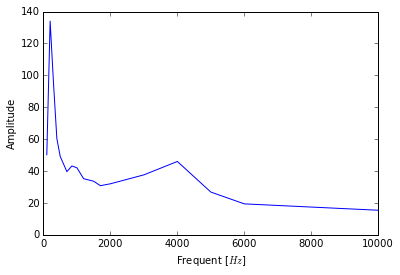
\includegraphics[width=165mm]{amplitude_gross.png}
\caption{Amplitude Lautsprecher gross}
\label{img:AmplitudeLGross}
\end{figure}

\begin{figure}[H]
\centering
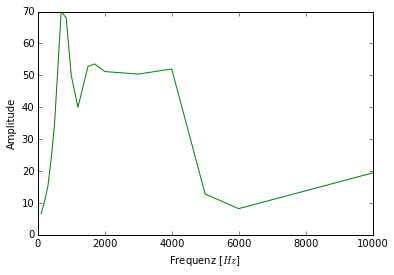
\includegraphics[width=165mm]{amplitude_klein.png}
\caption{Amplitude Lautsprecher klein}
\label{img:AmplitudeLklein}
\end{figure}

\begin{figure}[H]
\centering
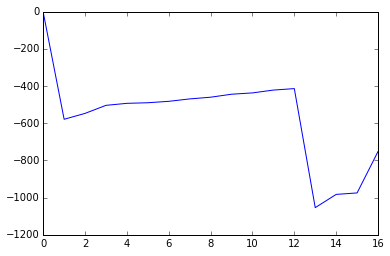
\includegraphics[width=165mm]{phase_gross.png}
\caption{Phase Lautsprecher Gross}
\label{img:phase_gross}
\end{figure}

\begin{figure}[H]
\centering
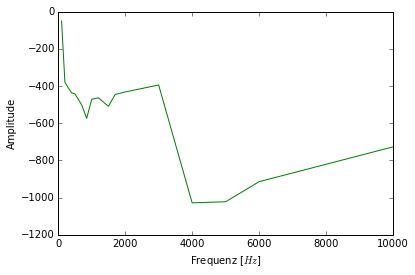
\includegraphics[width=165mm]{phase_klein.png}
\caption{Phase Lautsprecher klein}
\label{img:PhaseKlein}
\end{figure}

\begin{figure}[H]
\centering
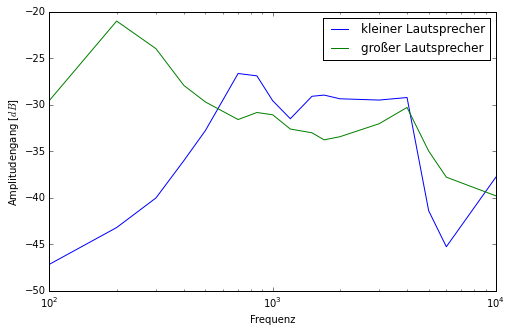
\includegraphics[width=165mm]{amplitudengang.png}
\caption{Bode-Diagramm Amplitudengang}
\label{img:BodeAmplitude}
\end{figure}

\begin{figure}[H]
\centering
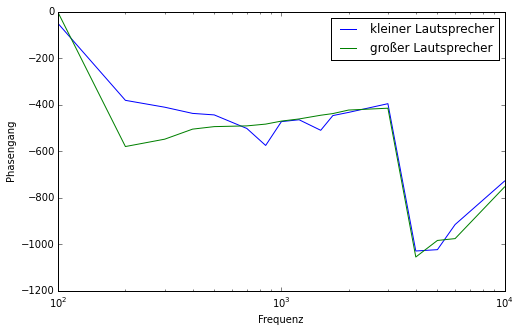
\includegraphics[width=165mm]{Phasengang.png}
\caption{Bode-Diagramm Phasengang}
\label{img:PhasenGang Bode-Diagramm}
\end{figure}

\section{Auswertung und Interpretation}
